\section{Zielsetzung}
In diesem Versuch soll die Schwingungs- und Schwebungsdauer gekoppelter Pendel untersucht werden.
Dabei werden gleichsinnige, gegensinnige und gekoppelte Schwingungen betrachtet.
\section{Theorie}
\label{sec:Theorie}
\subsection{Einzelnes Fadenpendel}
Zunächst wird ein einzelnes Fadenpendel, mit Länge $l$ und Masse $m$ betrachtet,
welches reibungsfrei Schwingen soll.
Bei einer Auslenkung wirkt die Gewichtskraft $\vec{F} = m \cdot \vec{a}$ entgegen der Bewegungsrichtung.
Dadurch entsteht ein Drehmoment $M = D_p \cdot \phi$, wobei $\phi$ den Auslenkwinkel und $D_p$ die Winkelrichtgröße beschreibt.
Die Bewegungsgleichung kann für kleine Auslenkwinkel ($\phi \leq 10°$) mit $\sin(\phi)= \phi$ vereinfacht werden.
Für die Bewegungsgleichung folgt:
\begin{equation*}
    J \cdot \ddot{\phi} + D_p \cdot \phi = 0.
\end{equation*}
Das Trägheitsmoment des Pendels wird mit $J$ beschrieben.
Eine harmonische Schwingung, also eine Bewegung, die nur mit Sinus und Kosinus Gliedern ausgedrückt werden kann, ist die Lösung dieser Bewegungsgleichung.
Für die Schwingungsfrequenz gilt:
\begin{equation*}
    \omega = \sqrt{\frac{D_p}{J}} = \sqrt{\frac{g}{l}}.
\end{equation*}
Somit ist die Schwingungsdauer bei der Kleinwinkelnäherung unabhängig von der Auslenkung und der Masse des Pendels.

\subsection{Gekoppeltes Fadenpendel}
Zwei Fadenpendel mit identischen Eigenschaften werden nun mithilfe einer Feder gekoppelt.
Dadurch entsteht ein zusätzliches Drehmoment auf jedes Pendel:
\begin{align*}
    M_1 &= D_F \cdot (\phi_2 -\phi_1),   &M_2 &= D_F \cdot (\phi_1 - \phi_2).
\end{align*}
Die Bewegungen der Pendel hängen somit voneinander ab und es folgt ein gekoppeltes Differentialgleichungssystem:
\begin{align*}
    J \cdot \ddot{\phi_1} + D \cdot \phi_1 = D_F \cdot (\phi_2 -\phi_1), \\
    J \cdot \ddot{\phi_2} + D \cdot \phi_2 = D_F \cdot (\phi_1 -\phi_2).   
\end{align*}
Hierbei wird die Schwingung des einzelnen Pendels auf der linken Seite und die Kopplung der Feder auf der rechten Seite beschrieben.
Das System kann durch geeignete Wahl der Auslenkungen entkoppelt und als Überlagerung von zwei Eigenschwingungen betrachtet werden.
Auch hier beschreibt eine harmonische Schwingung die Lösung der entkoppelten Bewegungsgleichungen mit den Schwingungsfrequenzen $\omega_1, \, \omega_2$
und den Auslenkwinkel $\alpha_1 , \, \alpha_2$.
Durch verschiedene Anfangsbedingungen $\alpha(t=0), \, \dot{\alpha}(t=0)$ werden unterschiedliche Schwingungen betrachtet.

\subsubsection{Gleichsinnige Schwingungen}
\label{subsubsec:gleich_theorie}
Die identischen Pendel werden um die gleichen Winkel ausgelenkt, $\alpha_1 = \alpha_2$.
Die rücktreibende Kraft wird nur durch die Gravitation erzeugt, somit kann die Kopplungsfeder auch entfernt werden, da sie keinen Einfluss auf die Bewegung hat.
Die Schwingungsfrequenz ist gleich der Eigenfrequenz der einzelnen Pendel und kann wie folgt beschrieben werden:
\begin{equation*}
    \omega_+ = \sqrt{\frac{g}{l}}.
\end{equation*}
Für die Schwingungsdauer gilt somit:
\begin{equation} \label{eqn:Tplus}
    T_+ = 2 \cdot \pi \sqrt{\frac{l}{g}}.
\end{equation}

\subsubsection{Gegensinnige Schwingung}
Bei der gegensinnigen Schwingung sind die zwei identischen, gekoppelten Pendeln um den gleichen Winkel entgegengesetzt ausgelenkt, $\alpha_1 = - \alpha_2$.
Dadurch verursacht die Kopplungsfeder auf beide Pendel eine gleich große, entgegengesetzte Kraft, wodurch eine symmetrische Schwingung erzeugt wird.
Für die Schwingungsfrequenz gilt:
\begin{equation*}
    \omega_- = \sqrt{\frac{g}{l} + \frac{2 \cdot K}{l}},
\end{equation*}
somit folgt für die Schwingungsdauer:
\begin{equation} \label{eqn:Tminus}
    T_- =2 \cdot \pi \cdot \sqrt{\frac{l}{g + 2 \cdot \kappa}}.
\end{equation}
Die Kopplungskonstante der Feder wird mit $\kappa$ beschrieben.

\subsubsection{Gekoppelte Schwingung}
Hierbei sind wieder zwei identische Pendel über eine Kopplungsfeder gekoppelt.
Ein Pendel soll zunächst ruhen, $\alpha_1 = 0$ und das andere wird ausgelenkt, $\alpha_2 \neq 0$.
Sobald das zweite Pendel beginnt zu schwingen, überträgt es seine Energie an das erste Pendel.
Während das zweite Pendel immer langsamer wird, bis es zur Ruhe kommt, nimmt das erste Pendel immer größere Amplituden auf, bis es das Maximum erreicht.
Die gerade beschriebene Bewegung bzw. der Energieübertrag widerholt sich.
Die sogenannte Schwebung beschreibt die Zeit zwischen zwei Stillständen eines Pendels.
Für die Schwebungsdauer $T_S$ gilt:
\begin{equation}\label{eqn:Ts}
    T_S = \frac{T_+ \cdot T_-}{T_+ - T_-},
\end{equation}
und für die Schwebungsfrequenz $\omega_S$:
\begin{equation} \label{eqn:ws}
    \omega_S = \omega_+ - \omega_-.
\end{equation}
Die Schwingungsdauer $T_+$ wird aus der gleichsinnigen und $T_-$ aus der gegensinnigen Schwingung ermittelt.
Die Kopplungskonstante $\kappa$ kann somit wie folgt bestimmt werden:
\begin{equation} \label{eqn:kappa}
    \kappa = \frac{\omega_-^2 - \omega_+^2}{\omega_-^2 - \omega_+^2} = \frac{T_+^2 - T_-^2}{T_+^2 + T_-^2}.
\end{equation}
\noindent
Alle genannten Schwingungsarten sind in \autoref{fig:Schwingungen} zu sehen.

\begin{figure}[h]
	\begin{subfigure}[b]{.33\linewidth}
	\centering
	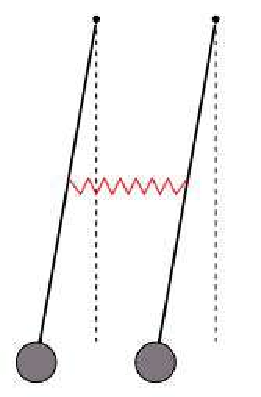
\includegraphics[height=3cm, keepaspectratio]{bilder/gleichsinnig.pdf}
	\caption{Gleichsinnige Schwingung.}\label{fig:gleich}
	\end{subfigure}%
	%
	\begin{subfigure}[b]{.33\linewidth}
	\centering
	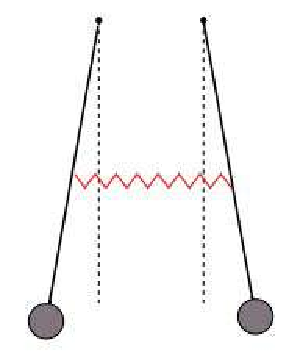
\includegraphics[height=3cm, keepaspectratio]{bilder/gegensinnig.pdf}
	\caption{Gegensinnige Schwingung.}\label{fig:gegen}
	\end{subfigure}
	%
	\begin{subfigure}[b]{.33\linewidth}
	\centering
	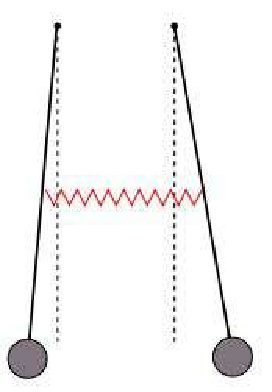
\includegraphics[height=3cm, keepaspectratio]{bilder/gekoppelt.pdf}
	\caption{Gekoppelte Schwingung.}\label{fig:gekoppelt}
	\end{subfigure}
	%
	% \begin{subfigure}[b]{.15\linewidth}
	% \centering    \Legende
	% \caption{Legende}\label{fig:leg}
	% \end{subfigure}
	%
	\caption{Die drei gekoppelten Schwingungsarten. \cite{anleitung}}
	\label{fig:Schwingungen}
	\end{figure}